\documentclass{article}
\usepackage{blindtext}
\usepackage[a4paper, total={6in, 8in}]{geometry}
\usepackage{breakurl}
\usepackage{amsmath}
\usepackage{amssymb}
\usepackage{caption}
%\usepackage{subcaption}
\usepackage{graphicx}
\usepackage{hyperref}
\usepackage{subfig}
\hypersetup{
    colorlinks=true,
    linkcolor=blue,
    filecolor=magenta,      
    urlcolor=cyan,
    pdftitle={Overleaf Example},
    pdfpagemode=FullScreen,
    }

\begin{document}


\title{PREDICT-AML: Personalized REsponse via Drug Interaction and Cellular Traits for Acute Myeloid Leukemia}
\author{Siddhi P. Jani, Halima Bensmail, Raghvendra Mall}
\date{}

\maketitle

\begin{figure}[!ht]
    \centering
    
\includegraphics[width=0.9\textwidth]{jtrm_images/Supp_Fig1.pdf}
    \caption{A. t-SNE plot showcasing uniform distribution of train and test set w.r.t. transcriptomic profiles. B. Best clustering performance obtained taking $150$ most variable genes. C. Optimal number of transcriptional subgroups identified at $k=3$. D. Distribution of the patient transcriptional profiles in the three subgroups visualized using PCA plot.}
    \label{fig:supp_fig1}
\end{figure}

\begin{figure}[!ht]
    \centering
    \includegraphics[width=0.95\textwidth]{jtrm_images/Supp_Fig2.pdf}
    \caption{A-G. Performance of machine learning models on test set. H-S. Performance comparison of different combinations of patient feature sets when used as input in the  CatBoost framework.}
    \label{fig:supp_fig2}
\end{figure}

\begin{figure}[!ht]
    \centering
    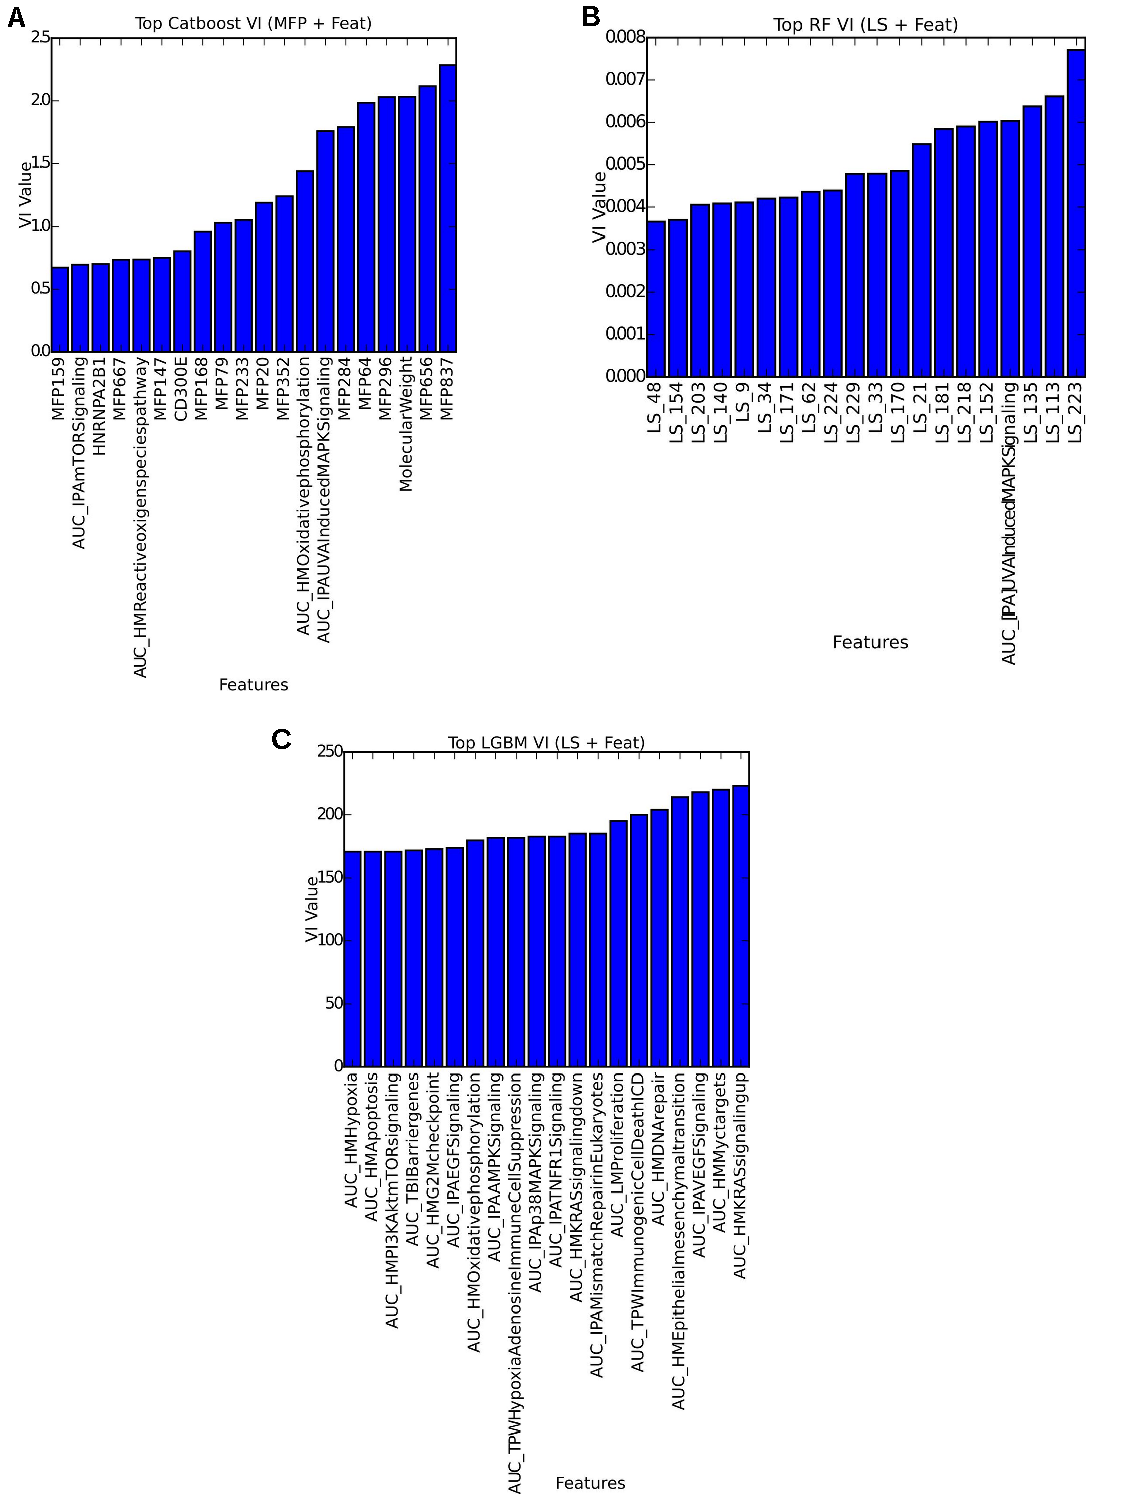
\includegraphics[width=0.95\textwidth]{jtrm_images/Supp_Fig3.pdf}
    \caption{A-C. Top 20 most important variables of the best tree-based models, CatBoost, Random Forest (RF) and LightGBM (LGBM) are highlighted. These models use either MFP or embedding representation (LS) for drugs together with molecular feature representation (Feat) for patients.}
\end{figure}

\begin{figure}[!ht]
    \centering 
    \subfloat[FigA][Association of scaled \textit{CD300E} expression with predicted AUC for top 10 drugs.]{
        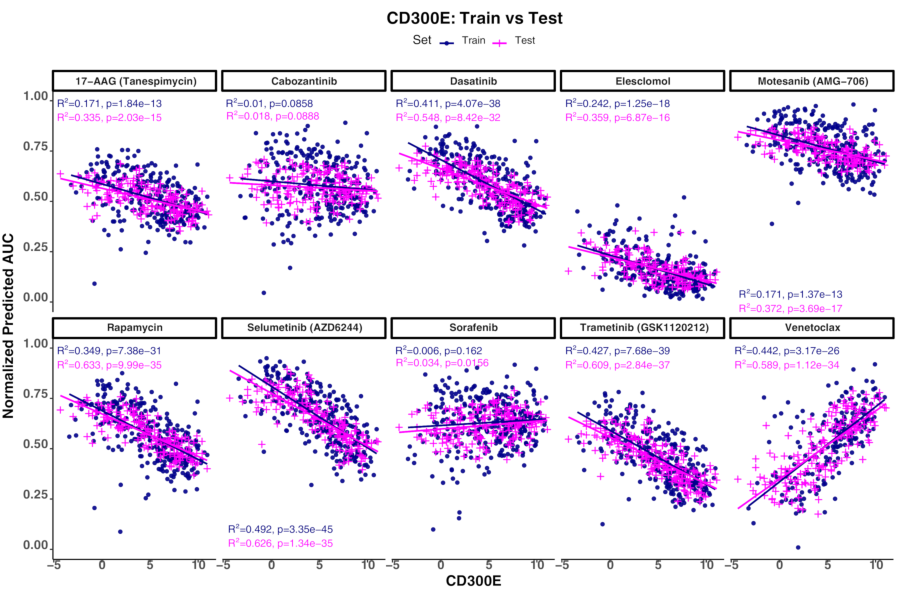
\includegraphics[width=0.93\textwidth]{jtrm_images/Supp_fig4.pdf-compressed_A.pdf}
    } 
    \qquad 
    \subfloat[FigB][Association of \textit{ARHGEF10L} expression with predicted AUC for top 10 drugs.]{
        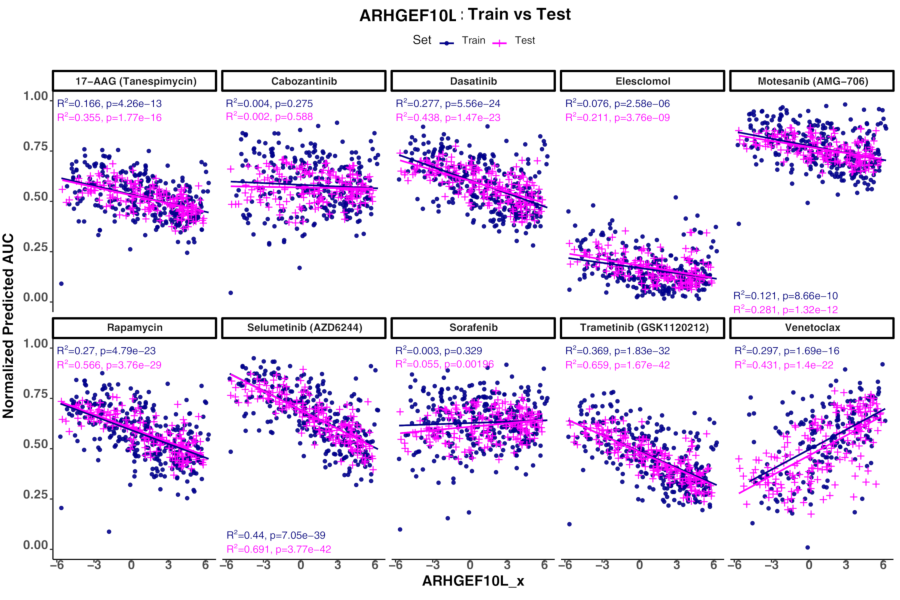
\includegraphics[width=0.93\textwidth]{jtrm_images/Supp_fig4.pdf-compressed_B.pdf}
    } 
\end{figure}

\begin{figure}[!ht]
  \ContinuedFloat 
  \centering 
  \subfloat[FigC][Association of scaled \textit{LGALS2} expression with predicted AUC for top 10 drugs]{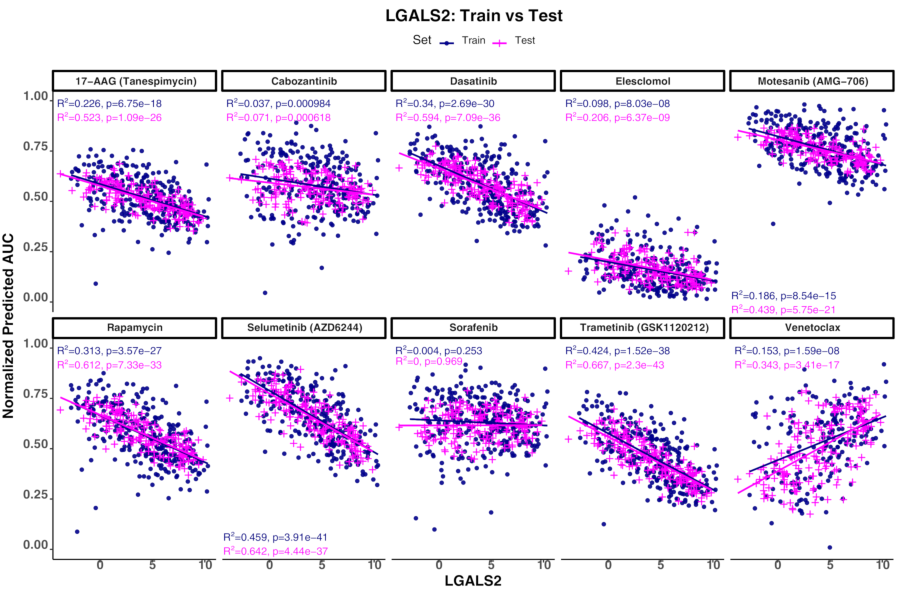
\includegraphics[width=0.93\textwidth]{jtrm_images/Supp_fig4.pdf-compressed_C.pdf}} 
  \qquad 
  \subfloat[FigD][Association of scaled M1 module enrichment with predicted AUC for top 10 drugs]{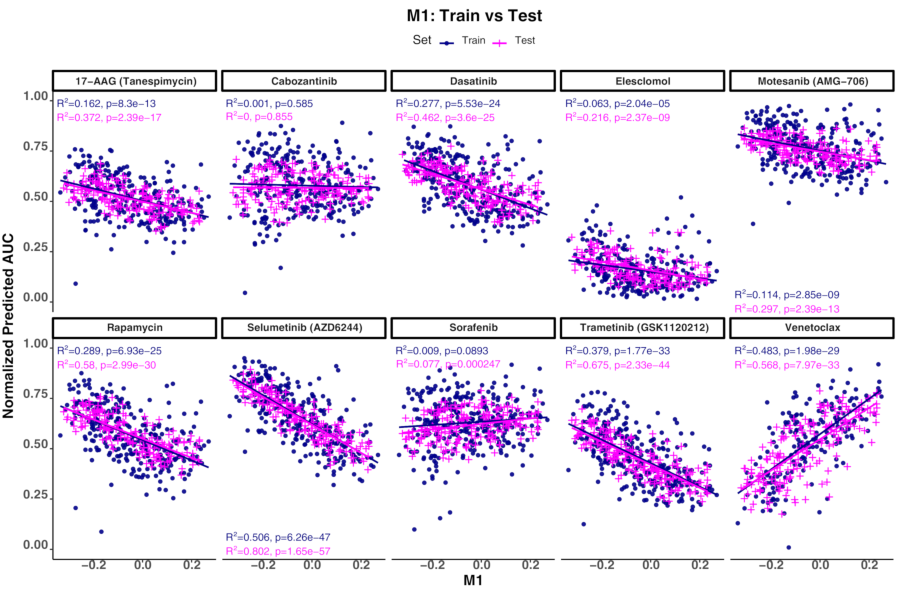
\includegraphics[width=0.93\textwidth]{jtrm_images/Supp_fig4.pdf-compressed_D.pdf}} 
\end{figure} 

\begin{figure}[!ht]
    \ContinuedFloat
    \centering
    \subfloat[FigE][Association of scaled \textit{VCAN} expression with predicted AUC for top 10 drugs]{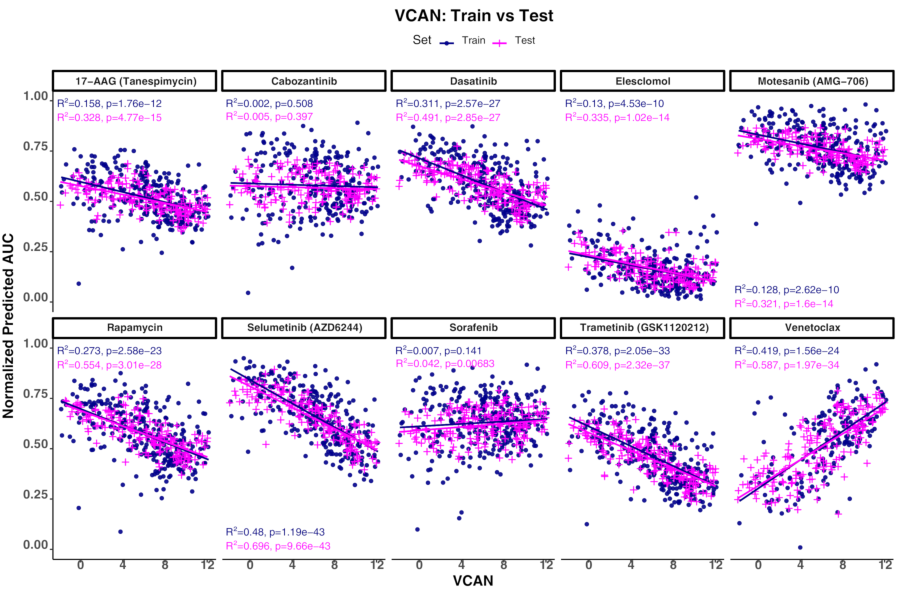
\includegraphics[width=0.93\textwidth]{jtrm_images/Supp_fig4.pdf-compressed_E.pdf}}
    \qquad
    \qquad
    \qquad
    \caption*{Figure 4: Linear regression analysis of top features significantly associated with predicted AUC score for top 10 drugs.}\label{fig:fig4}
\end{figure}

\end{document}